

\documentclass[11pt]{amsbook}

\usepackage{../HBSuerDemir}	% ------------------------


\begin{document}

% ++++++++++++++++++++++++++++++++++++++
\hPage{b2p1/74}
% ++++++++++++++++++++++++++++++++++++++

Accordingly  [$\lambda_{i}$, $\delta_{ij}$], [$\lambda\delta_{ij}$] are diagonal and scalar matrices respectively.

For a square matrix A = [$a_{ij}$], the symbols $\hAbs{A}$, det A, det[$a_{ij}$] are used to denote the determinant of A:
\begin{center}
$\hAbs{A}$=$\hAbs a_{ij}$ = det A = det[$a_{ij}$]
\end{center}
We note that if A is a non  square matrix, $\hAbs{A}$ is not defined.

\section{Operations with real matrices}

\subsection{Equality} The matrices [$a_{ij}$], [$b_{ij}$] are \underline{equal} if they are of the same size and corresponding elements are equal:
\begin{center}
 $[a_{ij}]_{mxn}$ = $[b_{ij}]_{mxn}$ $\iff$ $a_{ij}$ = $b_{ij}$ for all i, j.
\end{center}

\subsection{Addition} The \underline{sum} of two matrices $[a_{ij}]$, $[b_{ij}]$ of the same size is a matrix of the same size whose elements are the sums of their corresponding elements:
\begin{center}
 $[a_{ij}]_{mxn}$ + $[b_{ij}]_{mxn}$ = [$a_{ij}$ + $b_{ij}$]$_{mxn}$
\end{center}

\subsection{Multiplication by a scalar} The \underline{product} of a matrix with a scalar is a matrix of the same size obtained by multiplying every element of the matrix by that scalar:
\begin{center}
 $c[a_{ij}]$ = [c $a_{ij}]$ = [$a_{ij}$]c
\end{center}

\subsection{Subtraction} The difference A-B of two matrices A and B of the same size is the matrix A+ (- B):
\begin{center}
 $[a_{ij}]_{mxn}$ - $[b_{ij}]_{mxn}$ = [$a_{ij}$ - $b_{ij}$]$_{mxn}$
\end{center}

\subsection{Multiplication} The product AB is defined only when the number of columns in A is equal to the number of rows in B.

\end{document}  

%==== templates ====

%==== environments ====

%\begin{figure}[htb]
%	\centering
%	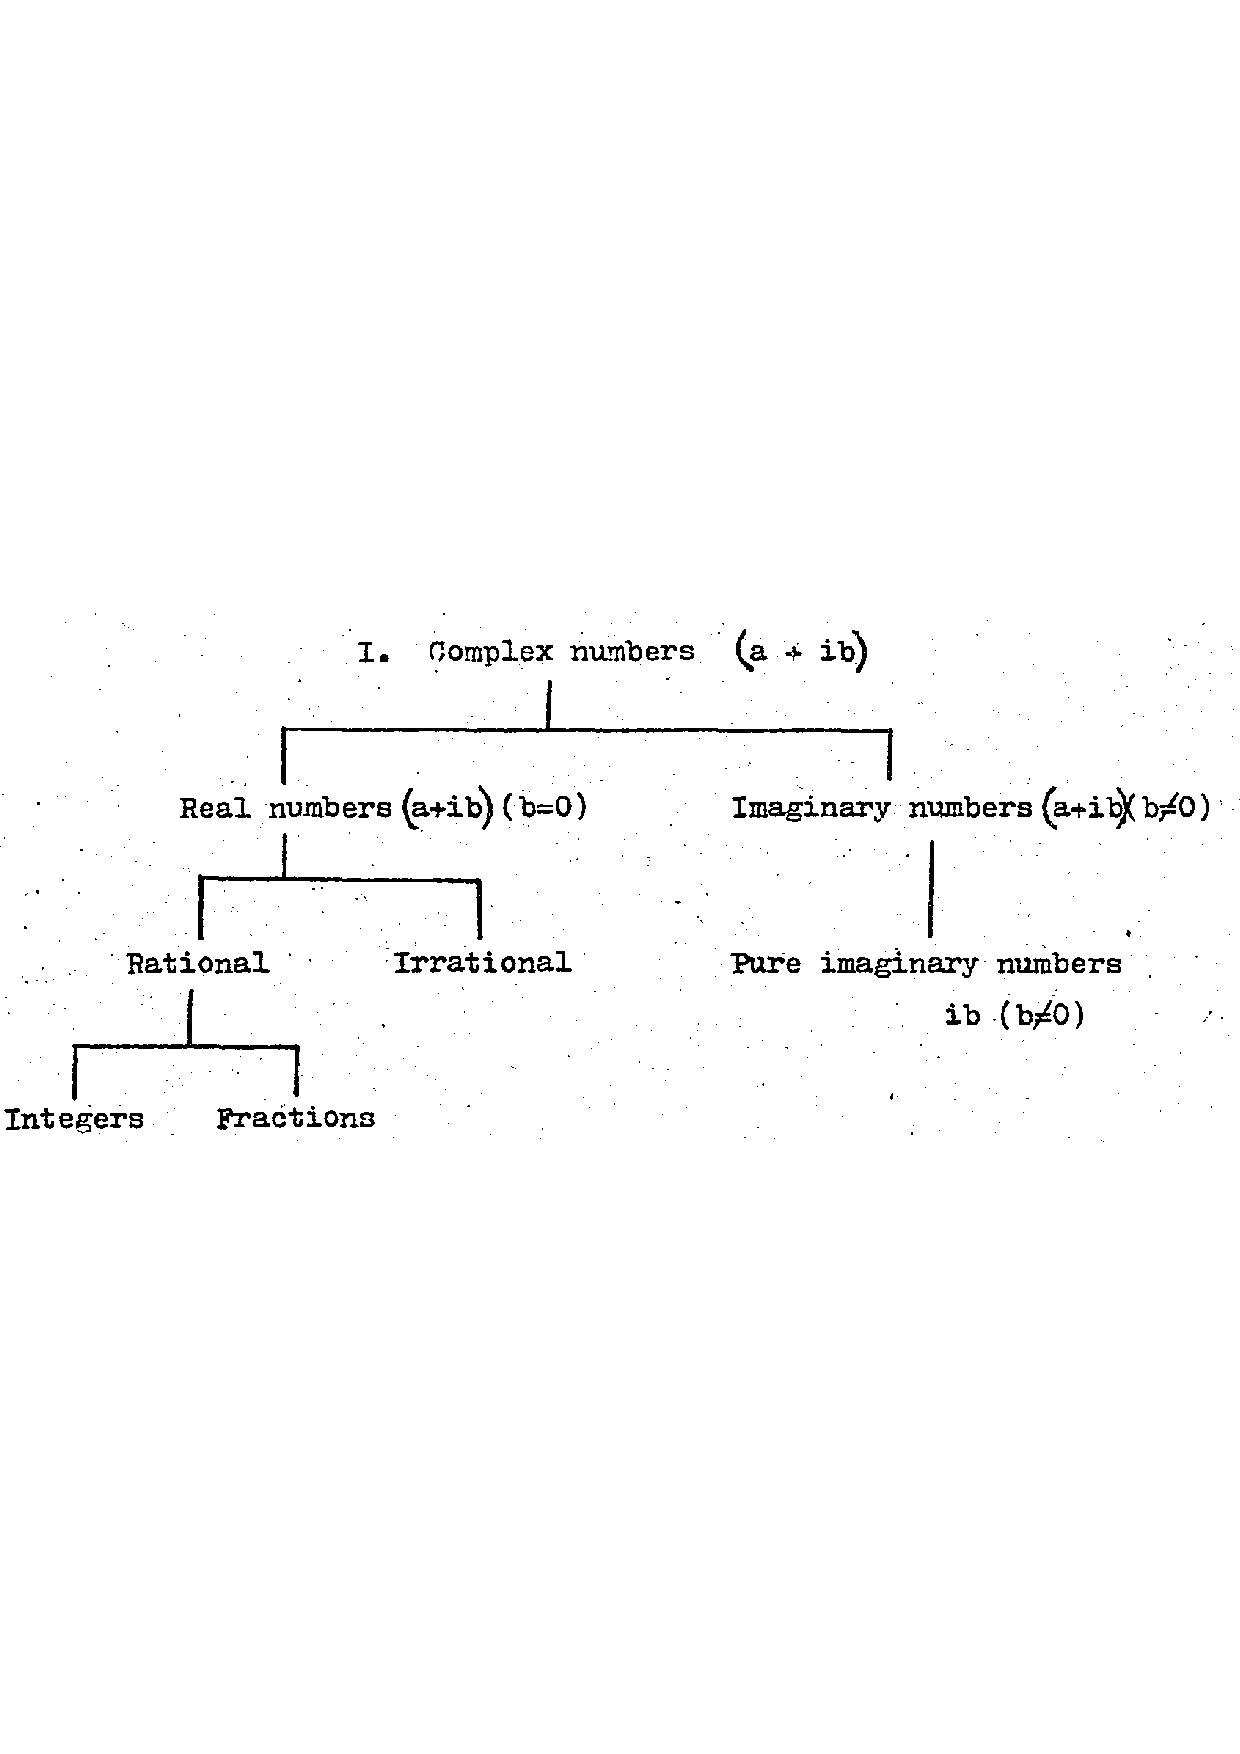
\includegraphics[width=0.9\textwidth]{images/SD-1-1p15A}
%	\caption{Classification of complex numbers}
%	\label{fig:classificationOfComplexNumbersA}
%\end{figure}

%\begin{center}
%\begin{tabular}{cc}
%\end{tabular}
%\end{center}

%\begin{exmp}
%\begin{hSolution}
%\end{hSolution}
%\end{exmp}

%\begin{hEnumerateAlpha}
%\end{hEnumerateAlpha}

%\begin{hEnumerateRoman}
%\end{hEnumerateRoman}

%$
%\begin{bmatrix}
%\end{bmatrix}
%$

%\frac{aaaa}{bbb}
%\frac{a_{n}}{b_{n}}
%\left( aaaa \right)
%\Longrightarrow

%\begin{multicols}{2}
%	bb
%\columnbreak
%	aa
%\end{multicols}
